\chapter{研究方法}\label{ch:method}

\section{实验框架}\label{sec:eval_framework}
% -- Purposes of Experiment -- %
目前,学界普遍认为自动评价指标和人类评价没有很强的相关性\upcite{HowNot},
但是不同指标之间的一致性似乎还没有得到充分的研究。
另一方面,生成式对话系统在不同数据集上的迁移能力(Transferability)
似乎是一个研究的比较少的问题。
开放领域的对话数据集所具有的大量噪音,
多样的话题和较弱的语法正确度对模型质量的影响似乎还没有引起学者们的重视。
通过实验,本文试图对上述问题进行初步的考察,
具体来说,本文试图回答以下问题:
\begin{enumerate}
    \item 模型的性能是否可以在不同数据集之间保持?
    \item 不同的指标在评价同一个数据集上的模型时有没有一致性?
    \item 模型和数据集,哪一个对得分的影响较大?
\end{enumerate}

% -- Terms and Definitions -- %
本文的实验涉及在多个数据集上训练多个模型,
然后用多种指标测量句子层面得分和系统层面得分。
表~\ref{tab:experiment_triples}~展示了实验所使用的模型,数据集和指标。
记模型的集合为$M$,数据集的集合为$D$,指标的集合为$S$,
为了避免术语上的模糊,本章指明:
一个模型$m \in M$指的是一种生成式模型的体系结构,而不是指一个训练好的模型实例。
一个数据集$d \in D$是指某个领域的全部对话的一个子集,它本身又被分为训练集,验证集和测试集三个子集,
一个指标$s \in S$是指一种能把上下文$c$,参考$r$和响应$\hat{r}$映射为一个实数的函数$f_s(c, r, \hat{r})$。
在不引起歧义时,在数据集$d$上训练指的是在$d$的训练集上训练,在数据集$d$上解码指的是在$d$的测试集上解码,
把模型$m$在数据集$d$上完成了训练的实例记为$(m, d)$。

% -- Framework -- %
如图~\ref{fig:framework}~所示,
本文的实验首先让每一个模型$m$在每一个数据集$d$上训练,
并让训练好的模型实例$(m, d)$在$d$上解码产生响应$r$,
然后再用每一个指标$s \in S$给$r$在句子层面打分,给$(m, d)$在系统层面打分,
分别得到$\lambda_{u}$和$\lambda_{s}$。
一组实验的最终结果是一个5元组$(m, d, s, \lambda_{s}, \lambda_{u})$,
表示在数据集$d$上训练的模型$m$在指标$s$
的评价下所得的系统层面得分$\lambda_s$和句子层面得分$\lambda_u$。

% -- Data Analysis -- %
本文用pandas\footnote{\url{https://pandas.pydata.org/}}装载实验数据,
用seaborn\footnote{\url{http://seaborn.pydata.org/}}进行数据可视化。
系统层面得分的数据由$(m, d, s, \lambda_s)$四元组组成,
$m, d, s$都是类别变量(Categorical Variable),
$\lambda_s$是数值变量(Numerical Variable)。
由于数据中的类别变量较多,
可视化采用面向类别变量的柱形图和箱体图。
本章用柱形图详细分析了不同模型在不同数据集和指标上的系统得分。
但是,某些模型在某些数据集上的得分过于接近,柱形图难以区分各个模型得分的高低。
于是本章分别从数据集和模型两个维度绘制了箱体图,加强了得分在某个维度上的区分程度。
这些箱体图作为辅助分析方法,放在附录~\ref{ch:dataset_system_dist}。

句子层面的得分$\lambda_u$是一个数值变量,
本章采用频数分布直方图进行分析。
一组待分析的句子层面得分是一个$n$维实值向量: $U_{(m, d, s)} = x_1, x_2, \dots, x_n$,
$n$是测试集的样本数,$(m, d, s)$是模型,数据集和指标组成的三元组,$x_i$是某个样本的得分。
句子层面得分可以看做是从一个分布的数学形式未知的总体的取样,
可以使用无参估计法之一的核密度估计(Kernel Density Estimation,KDE)来估计总体的分布。
句子层面得分比系统层面得分的粒度更细,数据也更多了,为了分析的效率,
本章选择了案例分析。
本章固定$m = m', d = d'$,分析所有指标在$(m', d')$上的情况。
附录~\ref{ch:metric_dist}~呈现了完整的数据。

\begin{table}[H]
    \centering
    \caption{实验对象一览}
    \label{tab:experiment_triples}
    \begin{tabular}{|r|m{0.6\textwidth}|}
        \hline
        模型 & HRED,LSTM,VHRED \\
        \hline
        数据集 & Ubuntu,OpenSubtitles,LSDSCC \\
        \hline
        指标 & BLEU,ROUGE,METEOR,Vector-Average,
        Vector-Extrema,Greedy-Matching,
        ADEM,PPL,Distinct-N \\
        \hline
    \end{tabular}
\end{table}

\begin{figure}[H]
    \centering
    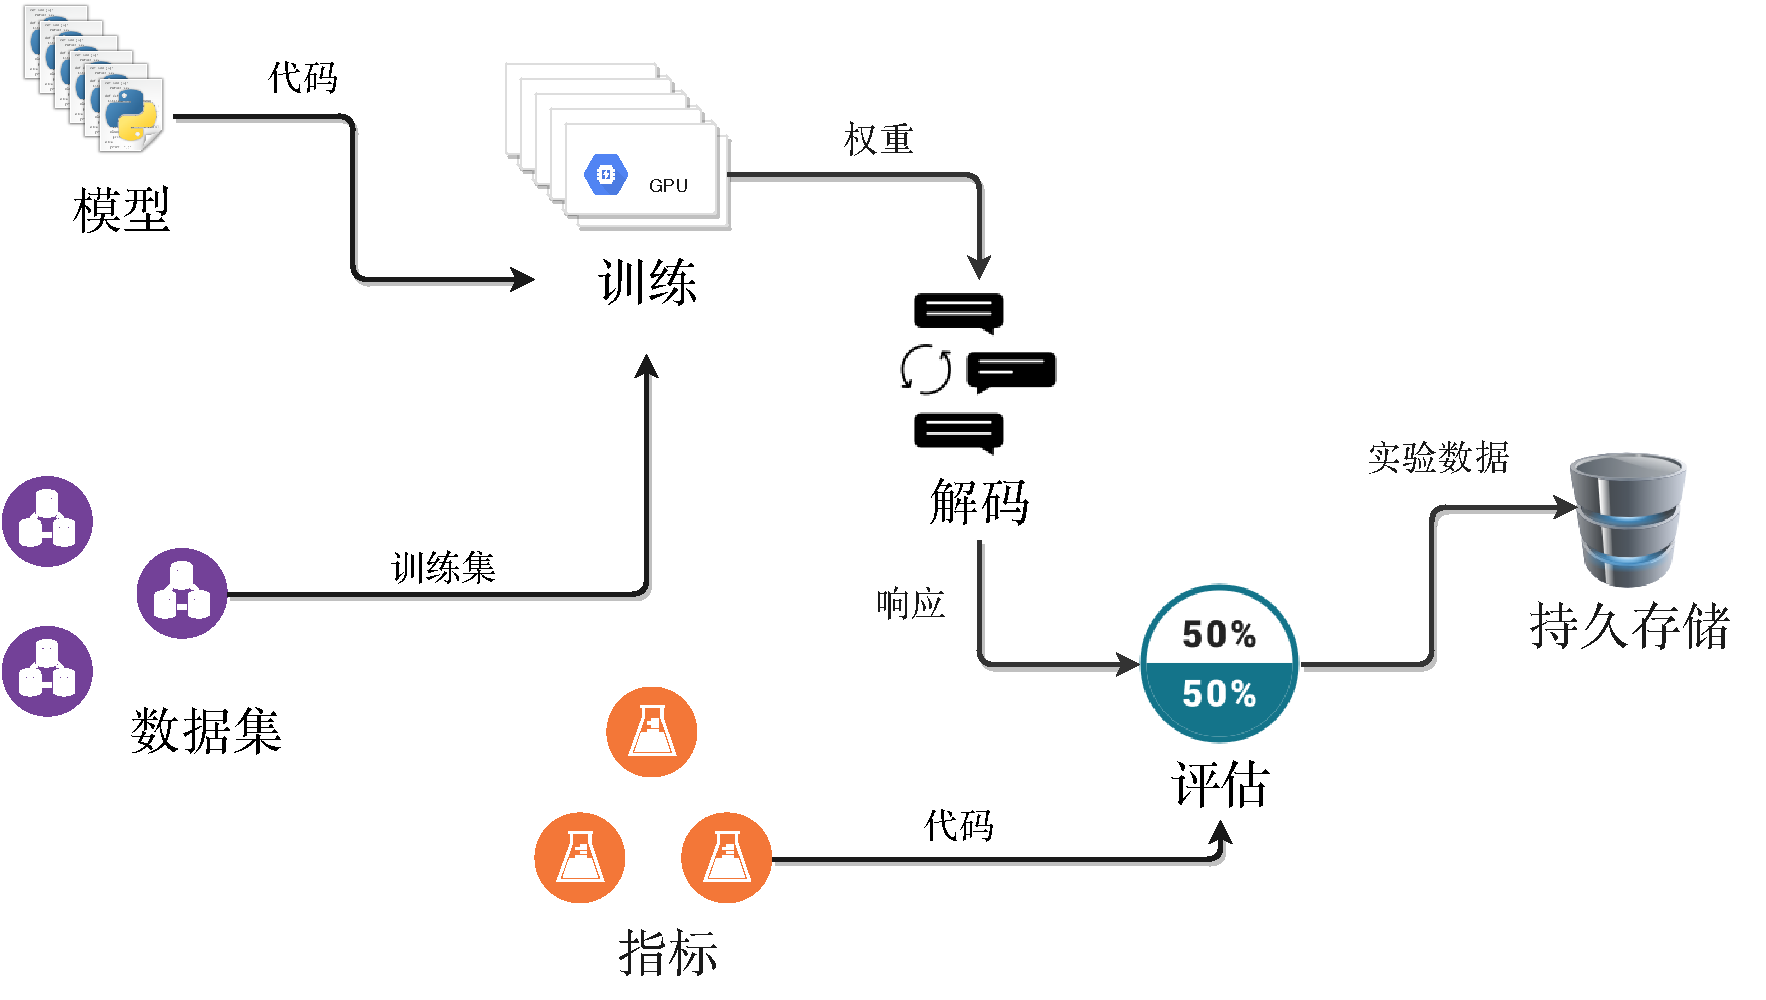
\includegraphics[width=0.8\textwidth]{figure/drawio/eval_v4.pdf}
    \caption{实验框架}
    \label{fig:framework}
\end{figure}

\section{模型选取}\label{sec:model_selection}
第~\ref{ch:related_work}~章已经介绍了生成式模型的基本概念和数据集、指标的基本情况。
和相对有限的数据集和指标相比,生成式模型的数量众多,
由于时间有限,
本文把考察的范围限定在基于Seq2Seq框架的生成式模型。
Serban等人在文献\cite{HRED,VHRED,MrRNN}
中提出HRED,VHRED和MrRNN模型,
它们是Seq2Seq框架在体系结构上的扩展。
这些模型都各具特色:
HRED能利用长期对话历史,
VHRED能捕捉对话中的不确定性(Uncertainty)和歧义性(Ambiguity),
MrRNN能生成带有高层次组合结构(Compositional Structure)的响应。
而且,HRED和VHRED都在Ubuntu对话数据集和
Twitter三元组数据集两个数据集上取得了不错的成绩,
说明它们在迁移能力方面是比较强的基线。
是否基于Seq2Seq框架和迁移能力是本章选择模型的两大依据,
HRED和VHRED很好的符合了本章的需求。

本章没有选取普通Seq2Seq模型作为基线,
而是选取了Serban等人使用的基线LSTM模型。
这是为了让实验设置尽可能接近Serban等人的设置,方便复现本文的实验;
本文把加入普通Seq2Seq模型作为以后的工作。
下面将详细介绍LSTM,HRED和VHRED三个模型。

% show the power of Serban
\subsection{LSTM模型}\label{subsec:LSTM}
LSTM是一种改进的循环神经网络,用于解决长时间依赖问题\upcite{LSTM}。
LSTM用多个门结构代替了普通RNN中隐藏矩阵$W_{hh}$。
\begin{align}
    f_t &= \sigma(W_f \cdot [h_{t-1}, x_t] + b_f) \\
    i_t &= \sigma(W_i \cdot [h_{t-1}, x_t] + b_i) \\
    \hat{C}_t &= \tanh(W_C \cdot [h_{t-1}, x_t] + b_C) \\
    C_t &= f_t \times C_{t-1} + i_t \times \hat{C}_t \\
    o_t &= \sigma(W_o \cdot [h_{t-1}, x_t] + b_o) \\
    h_t &= o_t \times \tanh(C_t)
    \label{eqn:LSTM_formula}
\end{align}

在公式~\ref{eqn:LSTM_formula}~中,
$x_t$是$t$时刻的输入,
$h_{t-1}$是$t-1$时刻的隐藏状态,
$C_{t-1}$是$t-1$时刻的单元状态(Cell State),
$f_t$是遗忘门(Forget Gate)的输出,
$i_t$是输入门(Input Gate)的输出,
$o_t$是输出门(Output Gate)的输出;
$W_f, W_i, W_o$是三个门的权重矩阵,
$b_f, b_i, b_o$是三个门的偏置向量,
$h_t$是通过一系列门运算后得出的$t$时刻的隐藏状态。
图~\ref{fig:LSTM_structure}~直观的
展现了LSTM内部各个门的连接方式和数据的流动,
LSTM正是通过这些复杂的门运算实现对较长的序列的记忆。
\begin{figure}[H]
    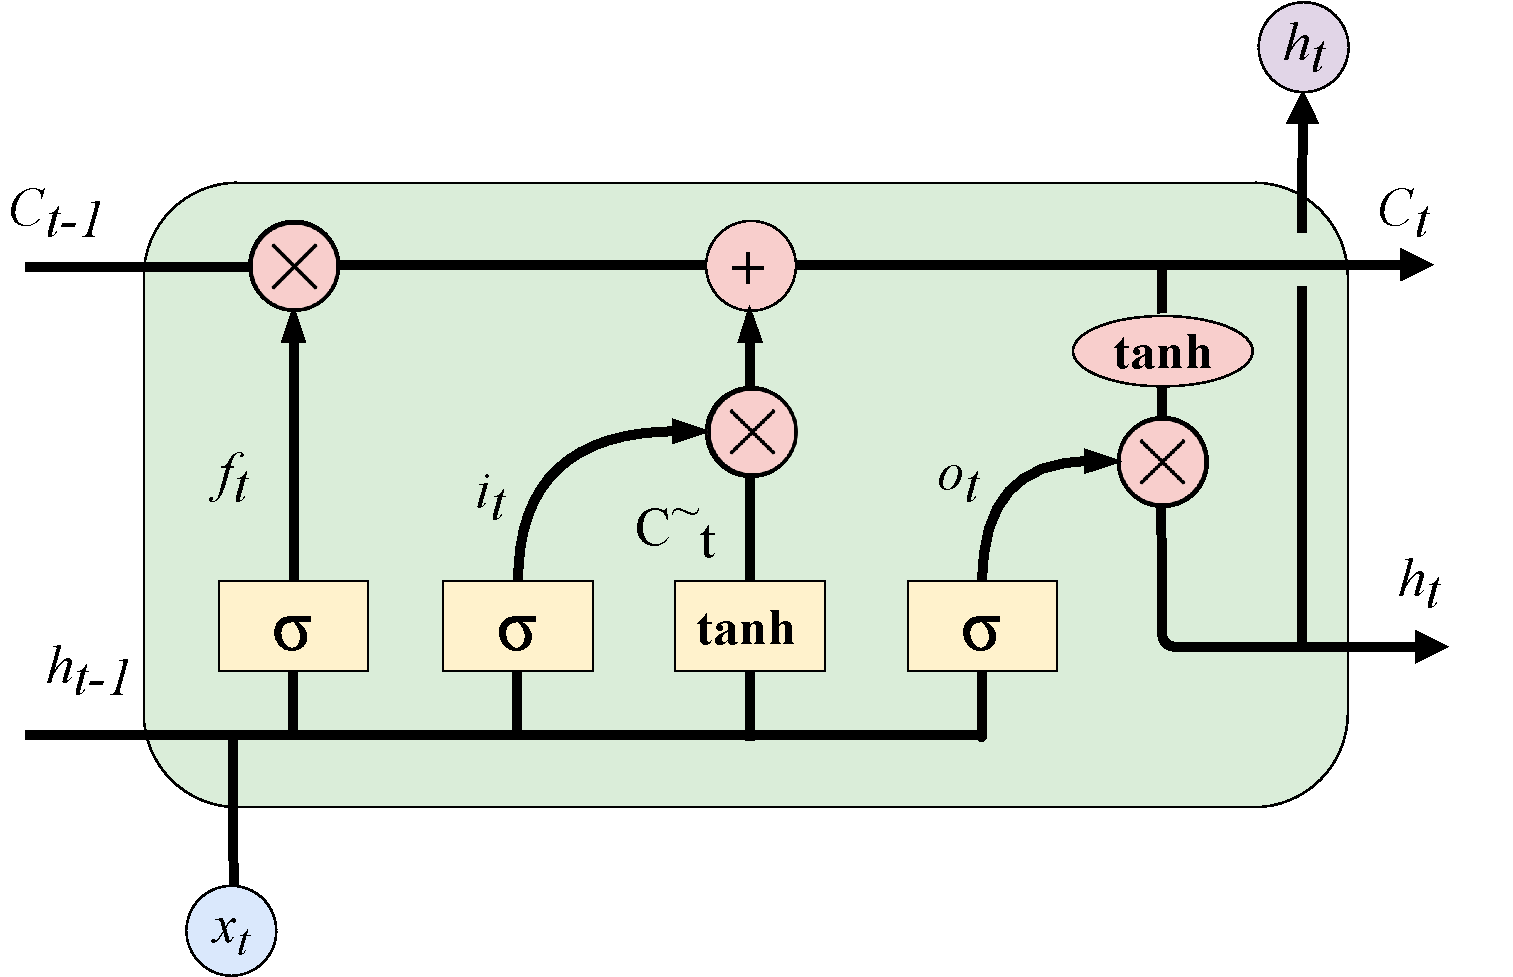
\includegraphics[width=0.5\textwidth]{figure/drawio/LSTM_v9.pdf}
    \centering
    \caption{LSTM内部结构图}
    \label{fig:LSTM_structure}
\end{figure}

如图~\ref{fig:LSTM_IO}~所示,
作为语言模型的LSTM与作为生成式模型的LSTM在数据的输出输出方式上有所不同。
作为语言模型时,输入数据为一个序列$X$,
模型需要重建概率$p(X)$,
在$t_0$时刻,模型输入一个特殊的句子开始符号(Start-of-Sentence),
在$t$时刻,模型的输入$x_t$是$t-1$时刻的输出$y_{t-1}$,
模型的输出$y_t$将和$X$序列的第$t$个元素$X_t$对比,并进行梯度下降。
作为生成式模型时,
输入数据是一对序列$(X, Y)$,
模型需要重建条件概率$p(Y|X)$,
在$t$时刻,模型的输入是$X$序列的第$t$个元素,
模型的输出$y_t$将和$Y$序列的第$t$个元素$Y_t$对比,并进行梯度下降。
本文的实验使用的是作为生成式模型的LSTM。
\begin{figure}[H]
    \begin{subfigure}{0.4\linewidth}
        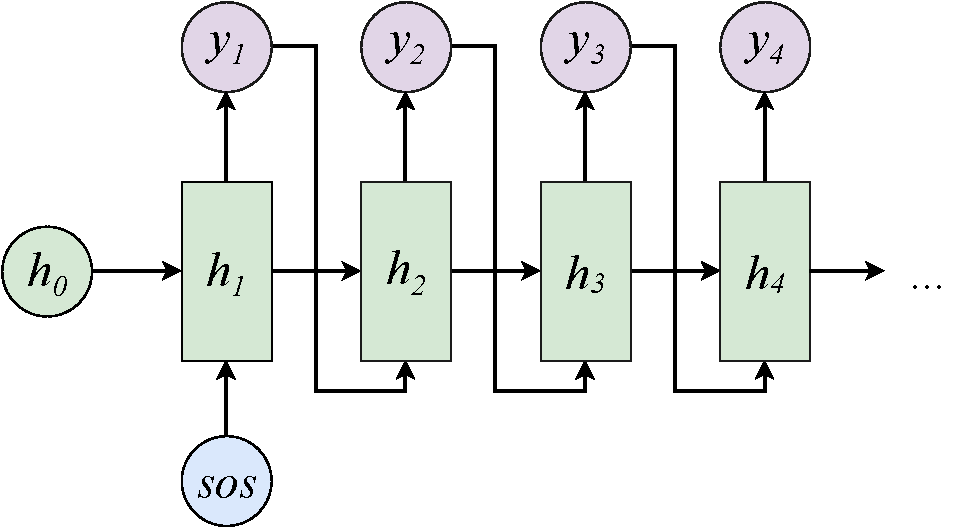
\includegraphics[width=\linewidth]{figure/drawio/RNNLM_lm_v2.pdf}
        \centering
        \caption{语言模型}
        \label{fig:RNNLM_}
    \end{subfigure}%
    \begin{subfigure}{0.4\linewidth}
        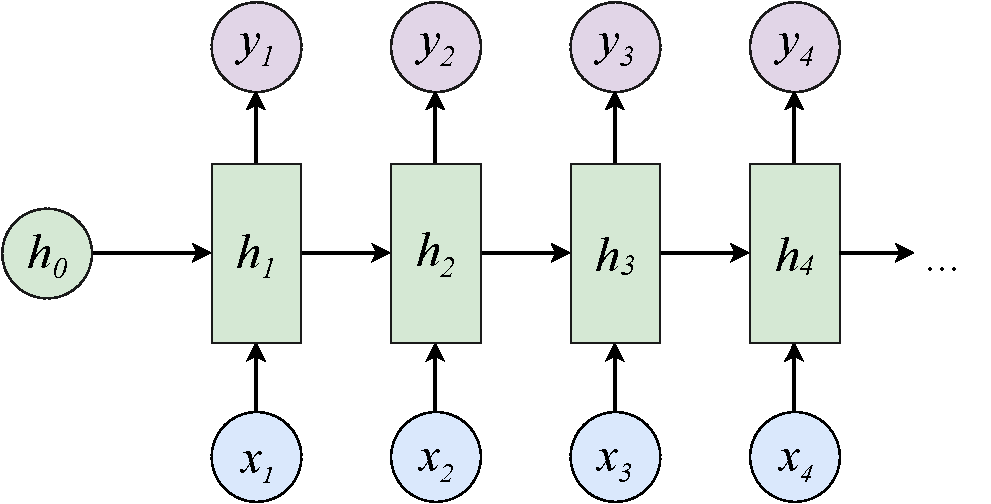
\includegraphics[width=\linewidth]{figure/drawio/RNNLM_generative_v1.pdf}
        \centering
        \caption{生成式模型}
        \label{fig:RNNLM_generative_v1}
    \end{subfigure}
    \centering
    \caption{LSTM模型的两种输入输出方式}
    \label{fig:LSTM_IO}
\end{figure}

\subsection{HRED模型}\label{subsec:HRED}
多层编解码器(Hierarchical Recurrent Encoder-Decoder,HRED)\upcite{hred-qs}
是一种能利用多轮对话结构的生成式模型。
它把一个对话看做一个两层序列结构,
一个对话$D$由$M$个句子组成:$D = \{ U_1, \dots, U_M \}$,
每个句子由$N_m$个单词组成:$U_m = \{ w_{m, 1}, \dots, w_{m, N_m} \}$。
\begin{figure}[H]
    \centering
    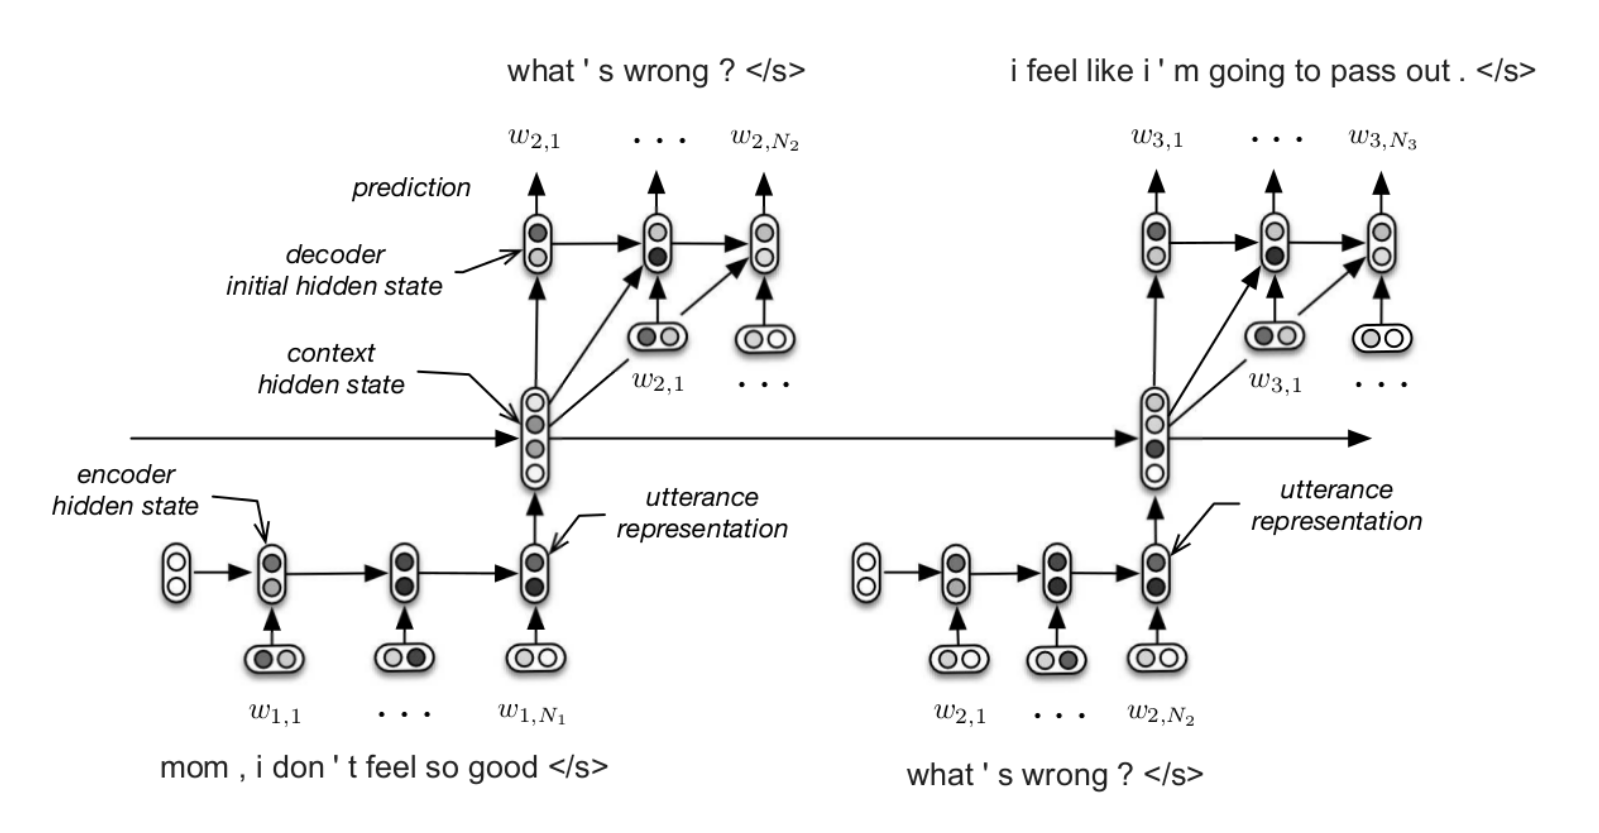
\includegraphics[width=\textwidth]{figure/HRED.png}
    \caption{HRED的计算图\upcite{HRED}}
    \label{fig:HRED}
\end{figure}

如图~\ref{fig:HRED}~所示,
HRED由三个部件组成:
句子编码器(Utterance Encoder)负责把每一个句子编码成一个固定长度的句子向量(Utterance Vector)$e_u$,
上下文编码器(Context Encoder)负责把$m$个句子向量$e_{u,1}, \dots, e_{u,m}$编码为一个对话向量(Dialogue Vector)$e_d$,
最后,句子解码器(Utterance Decoder)以对话向量$e_d$为输入,生成对话的下一个句子$U_{m+1}$。
本质上, 通过把对话分解为句子的序列, 把句子分解为单词的序列,
HRED估计了一个对话$D$的概率$P_{\theta}(D)$:
\begin{align}
    P_{\theta}(D) =
    P_{\theta}(U_1, \dots, U_M) = \prod_{m=1}^M P_{\theta}(U_m|U_{<m})
    = \prod_{m=1}^M \prod_{n=1}^{N_m} P_{\theta}( w_{m, n} |w_{m, <n}, U_{<m} )
\end{align}

$\theta$是HRED模型的参数,
$U_{<m}$表示$U_m$之前的句子序列,
$w_{m, <n}$表示第$m$个句子的第$n$个单词之前的单词序列。


\subsection{VHRED模型}\label{subsec:VHRED}
隐变量多层编解码器(Latent Variable Hierarchical Recurrent Encoder-Decoder,VHRED)是HRED的扩展,
它在句子解码器中加入了潜随机变量。
如图~\ref{fig:VHRED}~所示,
模型在生成响应时,除了生成对话向量$e_d$外,还产生一个随机变量$z_n$,
并把$z_n$和$e_d$连接到一起作为句子解码器的输入。
随机变量$z_n$能有效增加响应的多样性。
\begin{figure}[H]
    \centering
    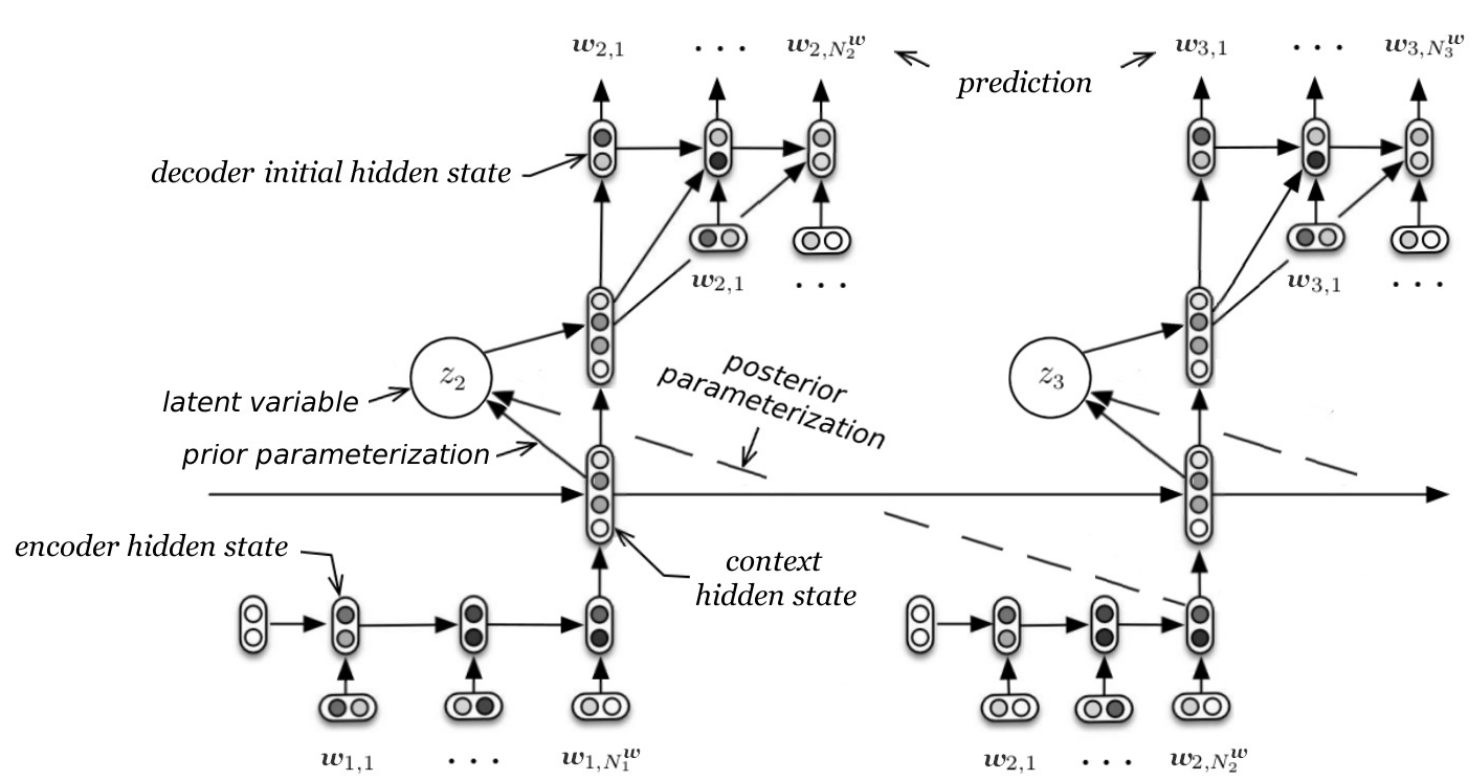
\includegraphics[width=0.8\textwidth]{figure/VHRED.png}
    \caption{VHRED的计算图\upcite{VHRED}}
    \label{fig:VHRED}
\end{figure}

$z_n$服从多元高斯分布$\mathcal{N}(\mu_{\text{prior}},
\Sigma_{\text{prior}})$,
$\mu_{\text{prior}}$是分布的均值,
$\Sigma_{\text{prior}}$是分布的协方差矩阵,
这些参数
由对话向量经过一个两层的前馈神经网络编码得到。
如公式~\ref{eqn:VHRED_random_variable}~所示,
对于一个对话$D = \{ U_1, \dots, U_M \}$,
每个句子
$U_m = \{ w_{m, 1}, \dots, w_{m, N_m} \}$,
模型通过$D$估计了分布$\mathcal{N}(\mu_{\text{prior}},
\Sigma_{\text{prior}})$。
如公式~\ref{eqn:VHRED_cond_prob}~所示,模型在条件概率
$P_{\theta}(U_n|U_1, \dots, U_{n-1})$
的条件部分加入了随机变量$z_n$,
它的作用可以理解为对话中的高层决策,
比如话题和情感,也可以理解为用随机变量模拟自然语言的对话中存在的
不确定性和歧义性。
模型的训练是通过变分推断(Variational Inference)实现的,
图中的后验参数(Posterior Parameterization)和训练有关。
\begin{align}
    P_{\theta}(z_n|{U}_1, \dots, U_{n-1}) = \mathcal{N}(\mu_{\text{prior}}(U_1, \dots, U_{n-1}), \Sigma_{\text{prior}}(U_1, \dots, U_{n-1}))
    \label{eqn:VHRED_random_variable} \\
    P_{\theta}(U_n|z_n, U_1, \dots, U_{n-1}) = \prod_{m=1}^{M_n}P_{\theta}(U_{n, m}|z_n, U_1, \dots, U_{n-1}, w_{n, 1}, \dots, w_{n, m-1})
    \label{eqn:VHRED_cond_prob}
\end{align}


\section{模型超参数设置}\label{sec:model_hparams}
% ------ Model setup ----------- %
在模型超参数方面,本文的设置大致和文献\cite{VHRED}相同。
本文用Adam\upcite{AdamOpt}来优化所有模型,
一个小批(Mini-batch)处理20个样本。
% -- Dimension of Word Embeddings -- %
本文在Ubuntu上使用维度是300的词嵌入,
在OpenSubtitles和LSDSCC上使用维度是400的词嵌入。
% -- Hidden Units of Utterance Encoder -- %
HRED和VHRED的句子编码器(Utterance Encoder)
在Ubuntu上使用500个隐藏单元,
在OpenSubtitles和LSDSCC上使用1000个隐藏单元。
% -- Hidden Units of Context Encoder -- %
HRED和VHRED的上下文编码器(Context Encoder)
在所有数据集上都使用1000个隐藏单元。
% -- Hidden Units of Utterance Decoder -- %
模型的句子解码器(Utterance Decoder)配置如
表~\ref{tab:utterance_decoder_config}~所示。
一般根据数据集的特点来设置不同RNN的隐藏单元数量,
在样本数多或者词汇表大的数据集上训练时,
隐藏单元数量会相应的增多。
% -- Direction of Utterance Encoder -- %
Ubuntu上的模型的句子编码器都使用了单向RNN,
而OpenSubtitles和LSDSCC上的模型的句子编码器则使用双向RNN。
% -- Gate Type of Utterance & Context Encoder -- %
所有模型的句子编码器和上下文编码器(如果有)都使用GRU作为门单元。
\begin{table}[H]
    \centering
    \caption{句子解码器的配置情况}
    \label{tab:utterance_decoder_config}
    \begin{tabular}{*{8}{l}}
        \toprule
        \midrule
        & \multicolumn{3}{c}{门单元类型} & & \multicolumn{3}{c}{隐藏状态单元数量} \\
        \midrule
        & HRED & LSTM & VHRED & & HRED & LSTM & VHRED \\
        \midrule
        LSDSCC & LSTM & GRU & GRU & LSDSCC & 1000 & 2000 & 1000 \\
        OpenSubtitles & LSTM & GRU & GRU & OpenSubtitles & 1000 & 2000 & 1000 \\
        Ubuntu & LSTM & LSTM & LSTM & 500 & Ubuntu & 2000 & 500 \\
        \bottomrule
    \end{tabular}
\end{table}

所有的模型都在一台Nvidia GTX上训练了至少1周。
模型收敛时的困惑度如表~\ref{tab:converged_perplexity}~所示。
与文献\cite{VHRED}不同的是,本文没有用预训练的HRED的参数来初始化对应的VHRED。
所有的模型都使用了梯度剪裁,阈值为1。
所有模型在Ubuntu上的学习率为0.0002,
在OpenSubtitles和LSDSCC上的学习率为0.0001。
在解码时,本文使用随机取样。
\begin{table}
    \centering
    \caption{模型收敛时的困惑度}
    \label{tab:converged_perplexity}
    \begin{tabular}{llll}
        \toprule
        \midrule
        & HRED & LSTM & VHRED \\
        \midrule
        LSDSCC & 32.9229 & 32.5599 & 37.7149 \\
        OpenSubtitles & 41.6392 & 34.2724 & 33.6867 \\
        Ubuntu & 39.1623 & 46.4055 & 40.2486 \\
        \bottomrule
    \end{tabular}
\end{table}

% -- Dataset Preprocessing -- %

\section{数据集选取}\label{sec:dataset_selection}
本文把注意力集中在三个数据集上:
Ubuntu对话数据集(Ubuntu Dialogue Corpus),OpenSubtitles,
LSDSCC数据集(A Large Scale Domain-Specific Conversation Corpus),
它们代表了三个常见的对话领域:技术支持,电影字幕和在线论坛。

% --------- Ubuntu ---------- %
Ubuntu对话数据集(下文简称Ubuntu)
是Lowe等人从Freenode IRC网络的Ubuntu板块的聊天日志\footnote{\url{https://irclogs.ubuntu.com/}}
中获取的技术性两人多轮对话。
这个数据集包含了大量技术符号,比如路径,命令,URL,还有笔误(Typo),缩写(Abbreviation)和俚语(Slang)。
它的样本数量多达930,000(接近1M),庞大的数据量为数据驱动的模型提供了极佳的试验场。
它的多轮特性为模型提供了更长的上下文,有助于模型生成更有意义的响应。

% --------- OpenSubtitles -------- %
OpenSubtitles是开源双语数据集项目(The Open Parallel Corpus,OPUS)的一部分。
它是从一个人们可以自由上传和下载电影字幕的网站\footnote{\url{http://www.opensubtitles.org}}的数据库中获取的,
庞大而充满噪音的开放领域数据集,对话数量高达80M。
由于OPUS的目的是收集机器翻译所需要的双语数据集(Parallel Corpus),OpenSubtitles也是一个双语数据集,
它里面并没有对话数据集所需要的轮信息(Turn Information),
而且也没有区分旁白,独白和对白。
Sordoni等人把OpenSubtitles用到对话领域\upcite{GoogleChatbot},
他们把相邻的两个句子分别视为消息和响应,并且每一个句子既是消息又是响应。
Li等人对OpenSubtitles也采用了类似的办法\upcite{MMI,persona,Future,DiverseBeam,
Distill,deep_RL,Adversarial}。

% --------- LSDSCC ------------- %
大规模特定领域对话数据集(A Large Scale Domain-Specific Conversational Corpus,LSDSCC)
是一个特定领域的单轮对话数据集\upcite{LSDSCC}。
它的训练集包含738,095个样本;它的词汇表比较大,达到了50K。
作者从Reddit的电影板块\footnote{\url{https://www.reddit.com/r/datasets}}中获取原始数据,
设计了一套尽可能保留语料信息的清理程序,还使让人类评价员对消息和响应的相关度进行评价,
最终得到一个高质量的消息-响应对数据集(Query-Reply Pair Corpus)。
作者还用信息检索的方法构建了一个多重参考测评集,并基于此提出了一系列衡量响应多样性的指标。


\section{数据集预处理}
\label{sec:dataset_proprecessing}
本文使用的Ubuntu对话数据集直接来自Serban等人的项目
\footnote{\url{https://github.com/julianser/hed-dlg-truncated.git}},没有经过任何额外处理。
本文从Li等人的项目
\footnote{\url{https://github.com/jiweil/Neural-Dialogue-Generation.git}}
中获取了经过预处理的OpenSubtitles数据,并作了如下处理:
\begin{enumerate}
    \item 将其从整数的下标形式还原为字符串的单词形式;
    \item 将其词汇表文件\texttt{movie\_25000}转化为下标从0开始的 pickle\footnote{pickle是一个Python特有的序列化格式}格式。
    \item 用Serban等人的\texttt{convert\_text2dict.py}将训练集,
    测试集和开发集均转换为pickle格式;
    \item 选用OpenSubtitles中的轮数为3, 句子最短长度为6的dialogue3\_6格式作为实际使用的数据集;
    \item 从测试集随机抽取1\%的样本作为正式使用的数据集。
\end{enumerate}

LSDSCC也是一个经过预处理的数据集\footnote{\url{https://drive.google.com/file/d/1nbpbnhwNP14xAc4SAc1 NN5lvEr01dQb/view?usp=sharing}}。
由于它的词汇数量多达50K,为了使内存不至于溢出,本文将其词汇表裁剪至35000个最常见的单词。
此外,由于本文只使用单个参考的指标,因此对LSDSCC的测试集中的多个参考,本文只取第一个参考。
剩下的处理过程类似OpenSubtitles的处理。

表~\ref{tab:dataset_stats}~是三个数据集的训练集(左)和测试集(右)的一些统计数据。
从表中可以看到,OpenSubtitles的样本数量要远远超过其他两个数据集,
是Ubuntu的26倍, 是LSDSCC的16倍。
但是,从单词数量来看,OpenSubtitles超过另外两个数据集的倍数却小得多,
这是因为Ubuntu的每一个样本包含了多个句子,
其长度要远远超过OpenSubtitles的样本。
这也导致了Ubuntu的样本数量少于LSDSCC,但是单词数量却超过了LSDSCC。
\begin{table}[H]
    \centering
    \caption{数据集的统计数据}
    \label{tab:dataset_stats}
    \begin{tabular}{*{8}{l}}
        \toprule
        \midrule
        & \multicolumn{4}{c}{训练集} & & \multicolumn{2}{c}{测试集} \\
        \midrule
        数据集 & 词汇数量 & 样本数量 & 单词数量 & 轮数 & 数据集 & 样本数量 & 单词数量 \\
        \midrule
        Ubuntu & 20000 & 448833 & 45697699 & 多轮 & Ubuntu & 18920 & 2045082   \\
        OpenSubtitles & 23876 & 11771393 & 379346841 & 多轮 & OpenSubtitles & 14714 & 474074 \\
        LSDSCC & 35008 & 738095 & 32355628 & 单轮 & LSDSCC & 299 & 10914 \\
        \bottomrule
    \end{tabular}
\end{table}

% -- Metric Config -- %
\section{指标配置}\label{sec:metric_config}
本文尽可能使用业界公认的指标实现和推荐的指标参数。
和文献\cite{HowNot}一样,本文只考虑单轮对话,
并且每个系统输出响应都只有单个参考响应。
% -- BLEU -- %
本文使用NLTK\footnote{\url{https://www.nltk.org/}}提供的BLEU实现,
并且加入了平滑处理。
% -- ROUGE -- %
本文实现了的ROUGE的一个版本,并将准确率和召回率的比例设置为1:9,
因为在机器翻译领域,
召回率和人类评价的相关性比准确率高\upcite{METEOR}。
ROUGE-W的权重设置为1.2 。
% -- METEOR -- %
本文使用了METEOR的官方实现\texttt{meteor-1.5.jar},并且按照官方文档
\footnote{\url{http://www.cs.cmu.edu/~alavie/METEOR/README.html}}的说明,
加入对特定语言(英语)的正则化处理。
% -- PPL -- %
本文使用Serban等人的\texttt{evaluate.py}脚本测量模型的困惑度,
由于该程序对测试样本进行了随机取样,本文无法得知某个样本的确切得分,
所以只测得了系统层面的得分。
% -- EB -- %
关于词嵌入的指标,
本文改写了Serban等人的\texttt{embedding\_metrics.py},
使之能测量句子层面的得分;
和他们一样,本文使用在谷歌新闻数据集(Google News Corpus)上预训练的
word2vec词嵌入\footnote{\url{https://drive.google.com/file/d/0B7XkCwpI5KDYNlNUTTlSS21pQmM}}。
% -- ADEM -- %
关于ADEM指标,本文使用作者提供的代码库
\footnote{\url{https://github.com/mike-n-7/ADEM.git}}
和预训练模型\footnote{\url{https://drive.google.com/file/d/0B-nb1w_dNuMLY0Fad3N1YU9ZOU0/view?usp=sharing}}。
% -- Distinct-N -- %
本文实现了比较简单的Distinct-N指标。
本文还测量了响应的句子长度$\textit{\#words}$,
以观察它对不同指标的得分的影响。

\section{本章小结}\label{sec:method_conclusion}
本章详细介绍了实验的各项设置,包括模型的超参数和训练过程,
数据集的预处理操作和一些统计数据,以及指标的实现和参数选择。
在下一章中,本文将展示实验的结果并进行讨论。
